% !TeX root = ../main.tex

\section{容差合并}

\def\naive{\codeinline{python}{Naive}}
\def\treed{\codeinline{csharp}{Tree3d}}
\def\kdtree{\codeinline{python}{k-d Tree}}

\subsection{容差合并的重要性和问题}

容差合并是参数化设计中一个重要的步骤, 旨在解决由于建模过程中引入的误差和不精确性所导致的重复点的问题.
这一步骤通常发生在将参数化模型转化为实际产品的过程中.

容差合并的重要性在于以下方面:
\begin{itemize}
  \item \emph{精确性:} 容差合并能够确保设计模型的准确性和精确性.
        在参数化设计中, 由于建模过程中的操作误差和计算机近似等因素, 可能会导致重复点的出现.
        通过进行容差合并, 可以消除这些重复点, 从而提高模型的精确性和准确性.
  \item \emph{可视化:} 容差合并还有助于改善设计模型的可视化效果.
        重复点会在可视化过程中产生杂乱的效果, 使设计师难以准确地观察和理解模型的细节.
        通过容差合并, 可以使设计模型更加清晰, 整洁, 为设计师提供更好的可视化效果.
  \item \emph{优化操作:} 容差合并可以简化模型编辑和操作的过程.
        重复点存在时, 设计师需要额外的操作来清理和调整模型.
        而通过容差合并, 设计师可以更方便地进行模型编辑和操作, 提高工作效率.
\end{itemize}

然而, 容差合并也存在一些问题和挑战:
\begin{itemize}
  \item \emph{容差选择:} 选择合适的容差是容差合并过程中的一个关键问题.
        过小的容差可能会导致重要的模型特征丢失, 而过大的容差可能会导致不必要的模糊和模型失真.
        设计师需要根据具体的设计要求和实际情况来选择合适的容差.
  \item \emph{数据处理:} 容差合并需要对大量的数据进行处理和计算.
        当模型复杂度增加时, 计算量和处理时间也会增加.
        设计师需要采用高效的算法和合适的计算资源来处理和优化这些数据, 以提高容差合并的效率和效果.
  \item \emph{误删问题:} 容差合并可能会误删设计模型中的一些细节和特征.
        在合并过程中, 一些本应存在的点可能会被错误地删除.
        为了避免这种问题, 设计师需要进行仔细的检查和验证, 确保容差合并不会对设计模型产生负面影响.
\end{itemize}

综上所述, 容差合并在参数化设计中起着重要的作用.
它可以提高模型的精确性和可视化效果, 优化操作流程, 但也需要面对容差选择, 数据处理和误删等问题.

\subsection{朴素容差合并算法的原理, 复杂度和效率分析}

% """
% remove_duplicate_points

% Removes similar points from a list

% Inputs:
%     P (Point)  : list of points to clean
%     t (Number) : points closer than this distance will be combined

% \Thetautput:
%     Q (Point) : list of unique points
% """

% import itertools

% import rhinoscriptsyntax as rs

% def point_less(u, v):
%     u_coordinates = rs.PointCoordinates(u)
%     v_coordinates = rs.PointCoordinates(v)
%     return u_coordinates < v_coordinates

% removed = set()
% for u, v in itertools.combinations(P, 2):
%     if u in removed or v in removed:
%         continue
%     if not rs.PointCompare(u, v, tolerance=t):
%         continue
%     removed.add(v if point_less(u, v) else u)
% Q = [u for u in P if u not in removed]

% 假设你是一名资深的参数化软件研究员, 你正在撰写一篇关于 Rhino 和 Grasshopper 的实际应用的论文. 你实现了一个朴素的容差合并算法, 请根据上述代码和信息, 撰写 "朴素算法" 一小节. 要求语言符合学术规范, 分析算法的复杂度和效率, 分析算法的优劣.

本节将介绍一种朴素的容差合并算法, 该算法能够从一个给定的点列表中去除相似的点.
该算法的目的是通过合并距离小于给定阈值的点来减少点的数量.

\inputcode[
  label          = lst:remove-duplicate-points-naive,
  minted options = {
      firstline = 19,
    },
][remove\_duplicate\_points\_naive.py]{python}{../python/remove_duplicate_points_naive.py}

算法使用了 Rhino 和 Grasshopper 中的 \codeinline{python}{rhinoscriptsyntax} 库作为辅助工具.
通过使用此库中的函数可以轻松地获取和操作点的坐标.

算法的输入包括一个点列表 \codeinline{python}{P} 和一个阈值 \codeinline{python}{t}, 表示距离小于t的点将会被合并.
算法的输出是一个不包含重复点的新的点列表 \codeinline{python}{Q}.

首先, 我们初始化一个集合 \codeinline{python}{removed} 用于存储已经被移除的点.
接下来, 我们使用 \codeinline{python}{itertools} 库中的 \codeinline{python}{combinations} 函数对点列表P中的每一对点进行组合.
通过对每一对点进行比较, 我们可以判断它们是否相似.

在比较两个点的相似性时, 首先检查这两个点是否已经被移除.
如果其中一个点已经被移除, 则可以跳过此对点的比较.

如果两个点的距离小于给定的阈值 \codeinline{python}{t}, 则它们被认为是相似的.
在这种情况下, 我们将选择其中一个点添加到 \codeinline{python}{removed} 集合中.
为了保持结果的一致性, 我们根据一个自定义的 \codeinline{python}{point_less} 函数来选择保留哪个点.
该函数将比较两个点的坐标, 并返回一个布尔值表示哪个点的坐标较小.
根据返回的结果, 我们添加较小的点到 \codeinline{python}{removed} 集合中.

最后, 我们根据 \codeinline{python}{removed} 集合将点列表 \codeinline{python}{P} 筛选为新的点列表 \codeinline{python}{Q}.
具体而言, 我们遍历列表 \codeinline{python}{P} 中的每一个点, 并判断每个点是否在 \codeinline{python}{removed} 集合中.
如果点不在 \codeinline{python}{removed} 集合中, 则将其添加到新的点列表 \codeinline{python}{Q} 中.

该算法的时间复杂度为 $\Theta(n^2)$, 其中 $n$ 是输入点列表的长度.
因为算法使用了两个嵌套的循环来比较每一对点, 所以算法的效率在处理大型输入时可能较低.

然而, 该算法的优点在于其简单性和易于实现, 特别是在处理相对较小的点列表时是一种可行的选择.
此外, 该算法不需要对点列表进行排序, 因此可以在不影响结果的前提下保持点的相对顺序.

如果对于大型点列表而言, 效率是非常重要的需求, 那么更高效的算法可以使用空间来进行换取, 例如构建临近点的索引结构, 以减少比较操作的时间复杂度.
但是这种算法可能会更加复杂, 并且需要额外的空间来存储索引结构.

因此, 选择使用哪种算法取决于具体的需求和时间 / 空间权衡.
对于一些简单的应用场景, 朴素算法足够实现要求; 对于更复杂的情况, 可以进一步研究和实现更高效的算法.

% protected override void SolveInstance(IGH_DataAccess DA)
% {
%     List<Point3d> points = new List<Point3d>();
%     double tolerance = 0.01;
%     DA.GetDataList("Points", points);
%     DA.GetData("Tolerance", ref tolerance);
%     points.Sort((Point3d a, Point3d b) => a.CompareTo(b));
%     HashSet<Point3d> point_set = new HashSet<Point3d>(points);
%     Node3d<Point3d> tree = new Node3d<Point3d>(
%         converter: (Point3d pt, out double x, out double y, out double z) =>
%         {
%             x = y = z = 0.0;
%             TreeDelegates.Point3dCoordinates(pt, ref x, ref y, ref z);
%         },
%         region: new BoundingBox(points)
%     );
%     tree.AddRange(points);
%     for (int i = 0; i < points.Count; i++)
%     {
%         if (!point_set.Contains(points[i]))
%             continue;
%         while (true)
%         {
%             List<Index3d<Point3d>> neighbors = tree.NearestItems(
%                 locus: points[i],
%                 groupSize: 2,
%                 minimumDistance: 0.0,
%                 maximumDistance: tolerance
%             );
%             if (neighbors.Count < 2)
%                 break;
%             Index3d<Point3d> neighbor = neighbors[1];
%             if (points[i].DistanceTo(neighbor.Item) > tolerance)
%                 break;
%             point_set.Remove(neighbor.Item);
%             tree.Remove(neighbor);
%         }
%     }
%     DA.SetDataList("UniquePoints", point_set);
% }

% 假设你是一名资深的参数化软件研究员, 你正在撰写一篇关于 Rhino 和 Grasshopper 的实际应用的中文论文. 你实现了两种容差合并算法 (分别是朴素算法和上述代码中的算法), 请根据上述代码和信息, 撰写介绍上述代码的一小节 (不必再介绍朴素算法), 并给这一小节取一个合适的标题. 要求语言符合学术规范, 分析算法的复杂度和效率, 分析算法的优劣.

\subsection{基于近邻搜索的容差合并算法}

在本节中, 我们介绍一种基于近邻搜索的容差合并算法, 该算法可以有效地处理大量的点集, 以合并距离小于给定容差的重复点.
该算法利用了 Rhino 和 Grasshopper 的空间数据结构和查询功能, 以提高合并效率和准确性.

\inputcode[
  label          = lst:remove-duplicate-points-csharp,
  minted options = {
      firstline = 49,
      lastline  = 88,
    },
][RemoveDuplicatePoints.cs]{csharp}{../csharp/HelloGrasshopper/RemoveDuplicatePoints.cs}

该算法的输入是一个点集和一个容差值, 输出是一个去除重复点后的点集.
该算法的主要步骤如下:
\begin{enumerate}
  \item 将点集按照 \codeinline{csharp}{x}, \codeinline{csharp}{y}, \codeinline{csharp}{z} 坐标进行排序, 以便后续的查找和删除操作.
  \item 创建一个空的 \codeinline{csharp}{HashSet}, 用于存储最终的结果.
  \item 创建一个空间划分树 \codeinline{csharp}{Node3d}, 用于存储和查询点集中的点.
        该树使用 Rhino 的 \codeinline{csharp}{BoundingBox} 作为划分区域, 使用 \codeinline{csharp}{TreeDelegates.Point3dCoordinates} 作为坐标转换器.
  \item 将点集中的所有点添加到 \codeinline{csharp}{HashSet} 和空间划分树中.
  \item 遍历点集中的每个点, 如果该点已经被从 \codeinline{csharp}{HashSet} 中移除, 则跳过该点; 否则, 执行以下操作:
        \begin{enumerate}
          \item 使用空间划分树的 \codeinline{csharp}{NearestItems} 方法, 查找距离该点在容差范围内的最近的两个点 (包括该点本身).
          \item 如果只找到一个点 (即该点本身), 则说明该点没有重复点, 继续下一个点的遍历.
          \item 如果找到两个或更多的点, 则说明该点有重复点, 取第二个最近的点作为重复点, 并从 \codeinline{csharp}{HashSet} 和空间划分树中移除该重复点.
                然后重复这一步骤, 直到找不到更多的重复点为止.
        \end{enumerate}
  \item 将 \codeinline{csharp}{HashSet} 中剩余的点作为输出返回.
\end{enumerate}

该算法的时间复杂度主要取决于两个方面: 排序和查找.
排序的时间复杂度为 $\Theta(n \log{n})$, 其中 $n$ 是点集的大小.
查找的时间复杂度为 $\Theta(k \log{n})$, 其中 $k$ 是每个点的平均重复数.
因此, 总的时间复杂度为 $\Theta(k n \log{n})$.
相比于朴素算法, 该算法利用了空间划分树来加速查找过程, 避免了对整个点集的遍历, 从而提高了效率.

该算法的空间复杂度主要取决于 \codeinline{csharp}{HashSet} 和空间划分树所占用的空间.
\codeinline{csharp}{HashSet} 的空间复杂度为 $\Theta(n)$, 空间划分树的空间复杂度为 $\Theta(n)$.
因此, 总的空间复杂度为 $\Theta(n)$.
相比于朴素算法, 该算法没有使用额外的数组或列表来存储临时结果, 从而节省了空间.

该算法的优势在于可以处理大量的点集, 并且可以灵活地调整容差值.
该算法也可以很容易地扩展到其他类型的几何对象, 如线段, 曲线, 面等.
该算法的缺陷在于需要对输入进行排序, 这可能会改变原始数据的顺序; 另外, 该算法也依赖于 Rhino 和 Grasshopper 的内置功能, 如果在其他平台上实现, 则可能需要自行编写相应的数据结构和查询方法.

\subsection{基于 k-d Tree 的容差合并算法}

% import sys
% from array import array

% import numpy as np
% from scipy.spatial import KDTree

% raw: array = array("f")
% raw.frombytes(sys.stdin.buffer.read())
% points: np.ndarray = np.array(raw[:-1]).reshape(-1, 3)
% tolerance: float = raw[-1]
% kdtree: KDTree = KDTree(data=points)
% results: set[int] = set(range(points.shape[0]))
% for i in np.lexsort(keys=points[:, ::-1].transpose()):
%     if i not in results:
%         continue
%     duplicates: set[int] = (
%         set(kdtree.query_ball_point(x=points[i], r=tolerance)) & results
%     )
%     min_id: int = min(duplicates, key=lambda x: tuple(points[x]))
%     results -= set(duplicates)
%     results.add(min_id)

% 假设你是一名资深的参数化软件研究员, 你正在撰写一篇关于 Rhino 和 Grasshopper 的实际应用的中文论文. 你实现了两种容差合并算法 (分别是朴素算法和上述代码中的算法), 请根据上述代码和信息, 撰写介绍上述代码的一小节 (不必再介绍朴素算法), 并给这一小节取一个合适的标题. 要求语言符合学术规范, 分析算法的复杂度和效率, 分析算法的优劣.

在本节中, 我们介绍一种基于 k-d 树的容差合并算法, 该算法可以有效地处理大量的点云数据, 并在给定的容差范围内合并重复的点.
该算法的主要思想是利用 k-d 树的空间划分和近邻搜索的特性, 来快速地找出距离小于容差的点, 并将它们替换为最小的点 ID.
该算法的核心代码如 \cref{lst:remove-duplicate-points-core} 所示, 完整代码参见 \cref{lst:remove-duplicate-points}:

\inputcode[
  label          = lst:remove-duplicate-points-core,
  minted options = {
      firstline = 11,
      lastline  = 21,
    },
][remove\_duplicate\_points.py]{python}{../python/remove_duplicate_points_core.py}

该算法的时间复杂度为 $\Theta(n \log{n} + k n)$, 其中 $n$ 是点的数量, $k$ 是平均每个点的近邻数量.
该算法的空间复杂度为 $\Theta(n)$, 因为它只需要存储点云数据和 k-d 树结构.
相比于朴素的容差合并算法, 该算法有以下优势:
\begin{itemize}
  \item 该算法可以处理任意维度的点云数据, 而朴素算法只能处理二维或三维的情况.
  \item 该算法可以利用 k-d 树的高效近邻搜索, 避免了对所有点进行两两比较, 从而降低了时间复杂度.
  \item 该算法可以通过对点云数据进行排序, 保证了合并后的点 ID 是最小的, 从而避免了对点 ID 的重排.
\end{itemize}

该算法也有一些局限性, 例如:
\begin{itemize}
  \item 该算法需要构建 k-d 树结构, 这会增加一定的空间开销和预处理时间.
  \item 该算法对于容差较大或点云密度不均匀的情况, 可能会产生过度合并或漏合并的问题.
  \item 该算法对于点云数据中存在噪声或异常值的情况, 可能会影响合并结果的质量.
\end{itemize}

因此, 在使用该算法时, 需要根据具体的应用场景和数据特征, 选择合适的容差参数和预处理方法, 以达到最佳的效果.

\subsection{容差合并算法的性能比较}

\begin{figure}[htbp]
  \centering
  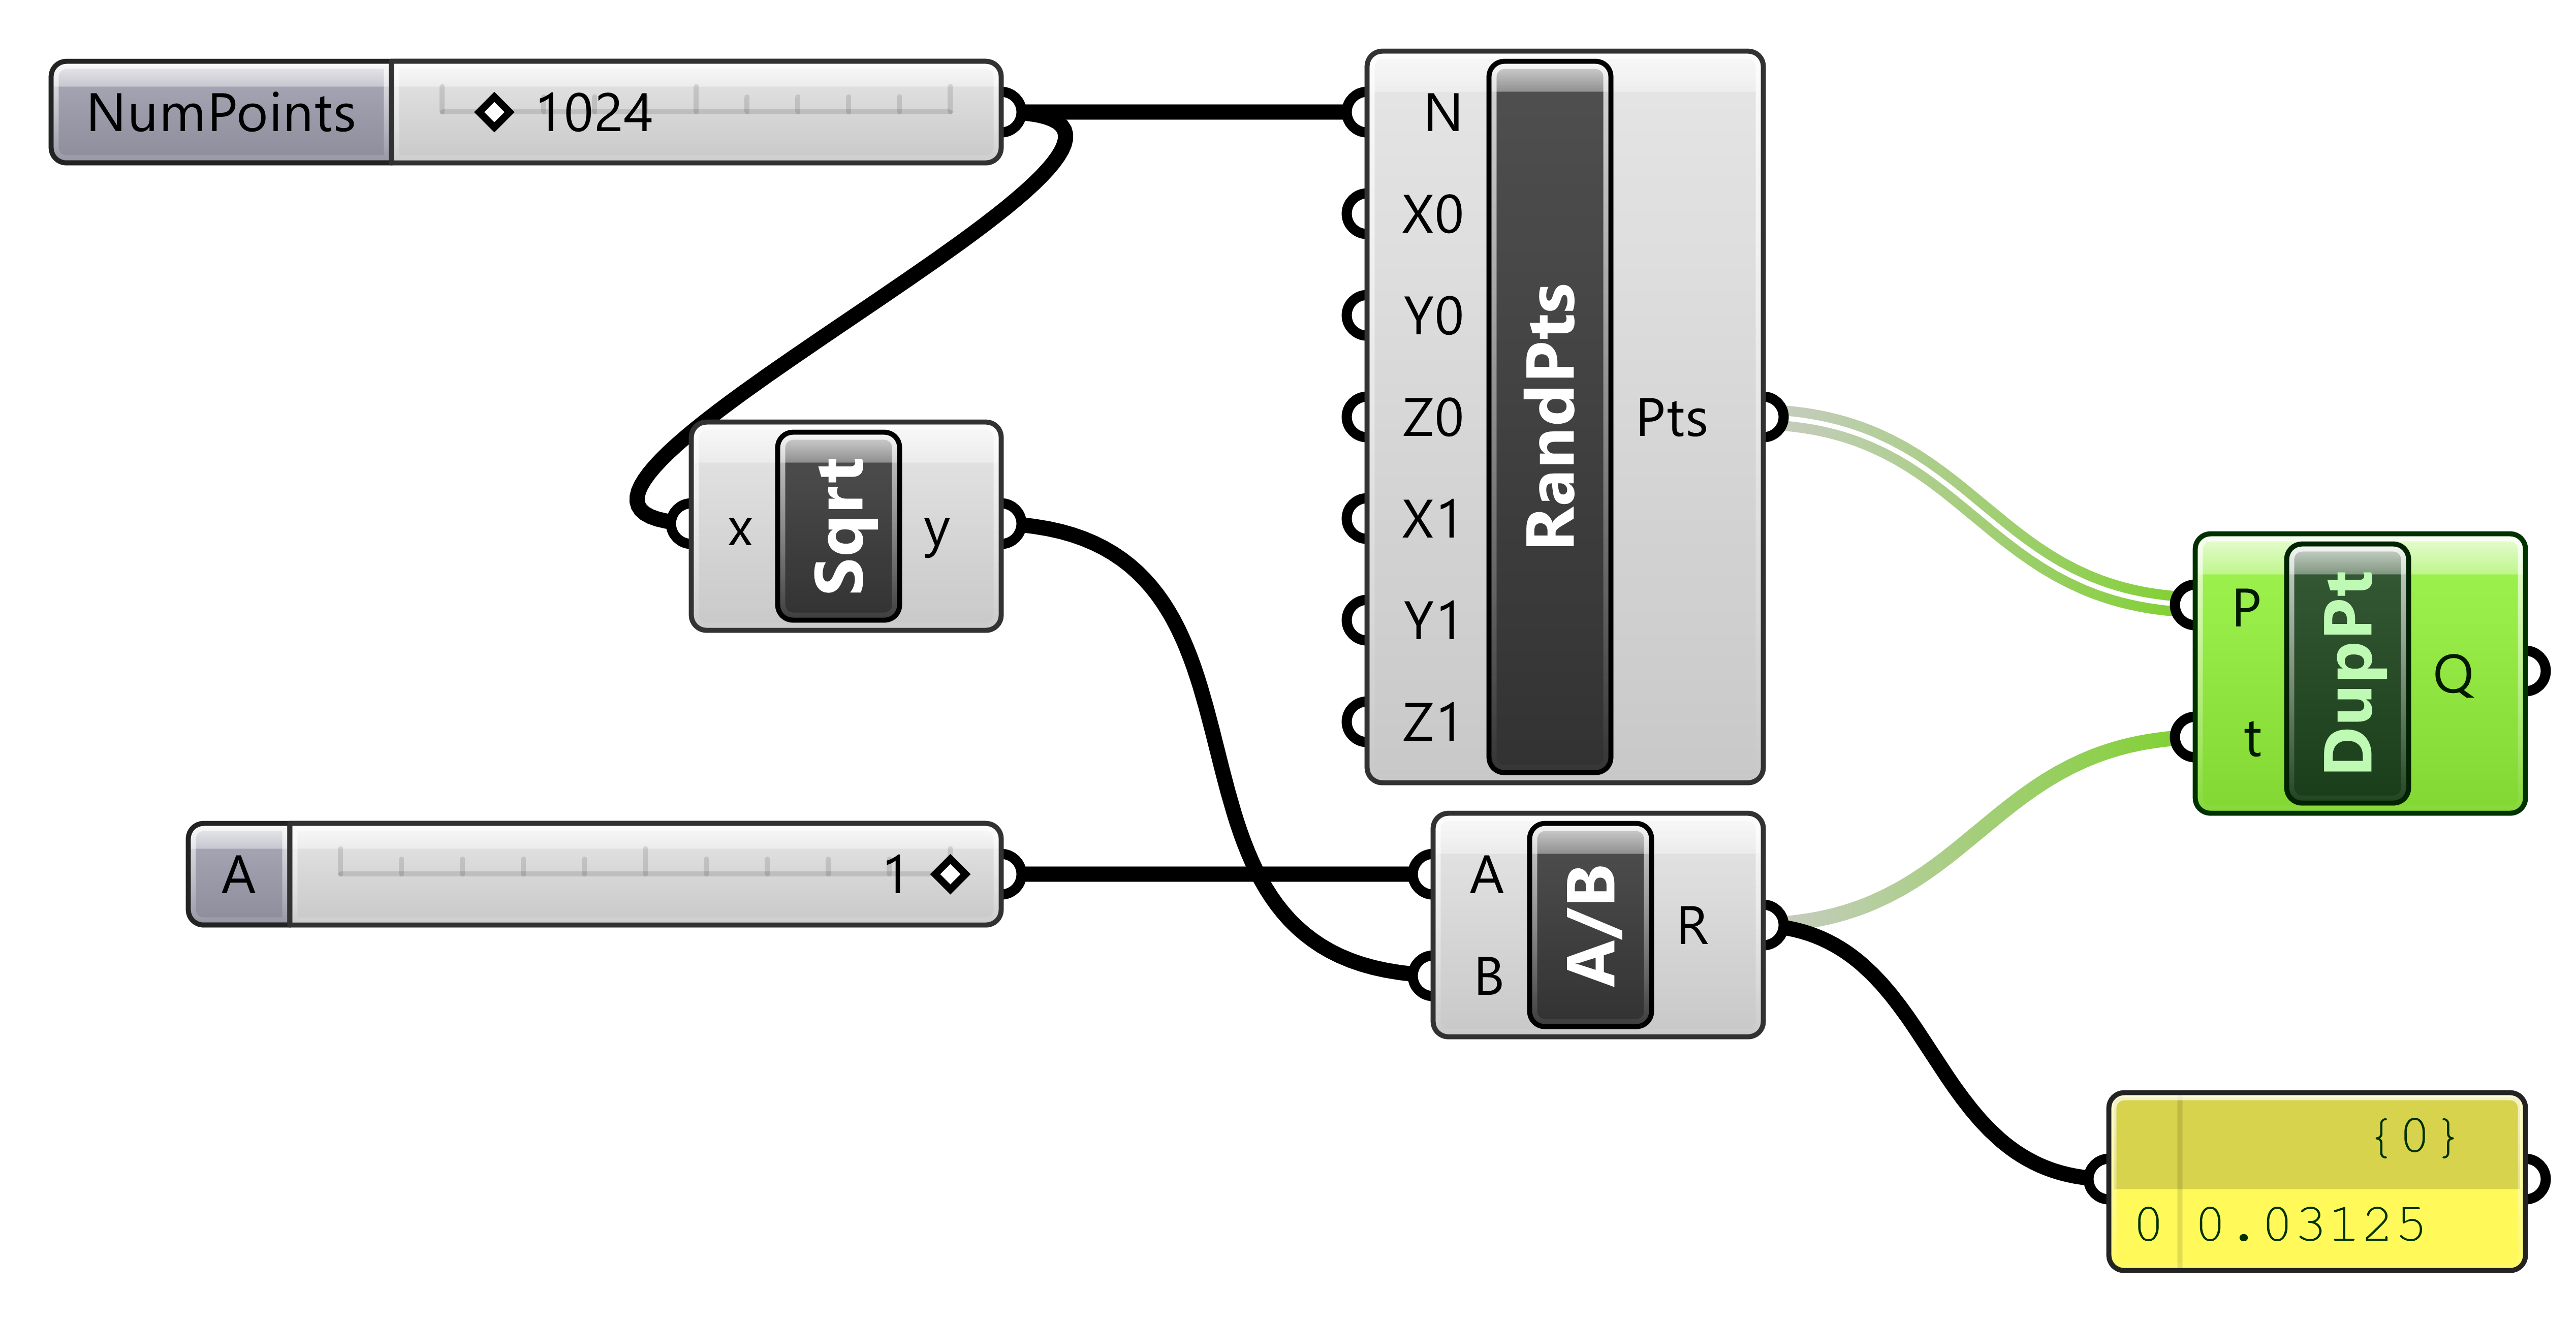
\includegraphics[width = 0.6 \linewidth]{remove-duplicate-points-gh.png}
  \caption{容差合并测试流程}
  \label{fig:benchmark-gh}
\end{figure}

\begin{figure}[htbp]
  \newtcbox{\keep}{
    bottom   = 0pt,
    colback  = green-1,
    colframe = green-6,
    coltext  = green-8,
    left     = 0pt,
    on line,
    right = 0pt,
    top   = 0pt,
  }
  \newtcbox{\remove}{
    bottom   = 0pt,
    colback  = red-1,
    colframe = red-6,
    coltext  = red-8,
    left     = 0pt,
    on line,
    right = 0pt,
    top   = 0pt,
  }
  \centering
  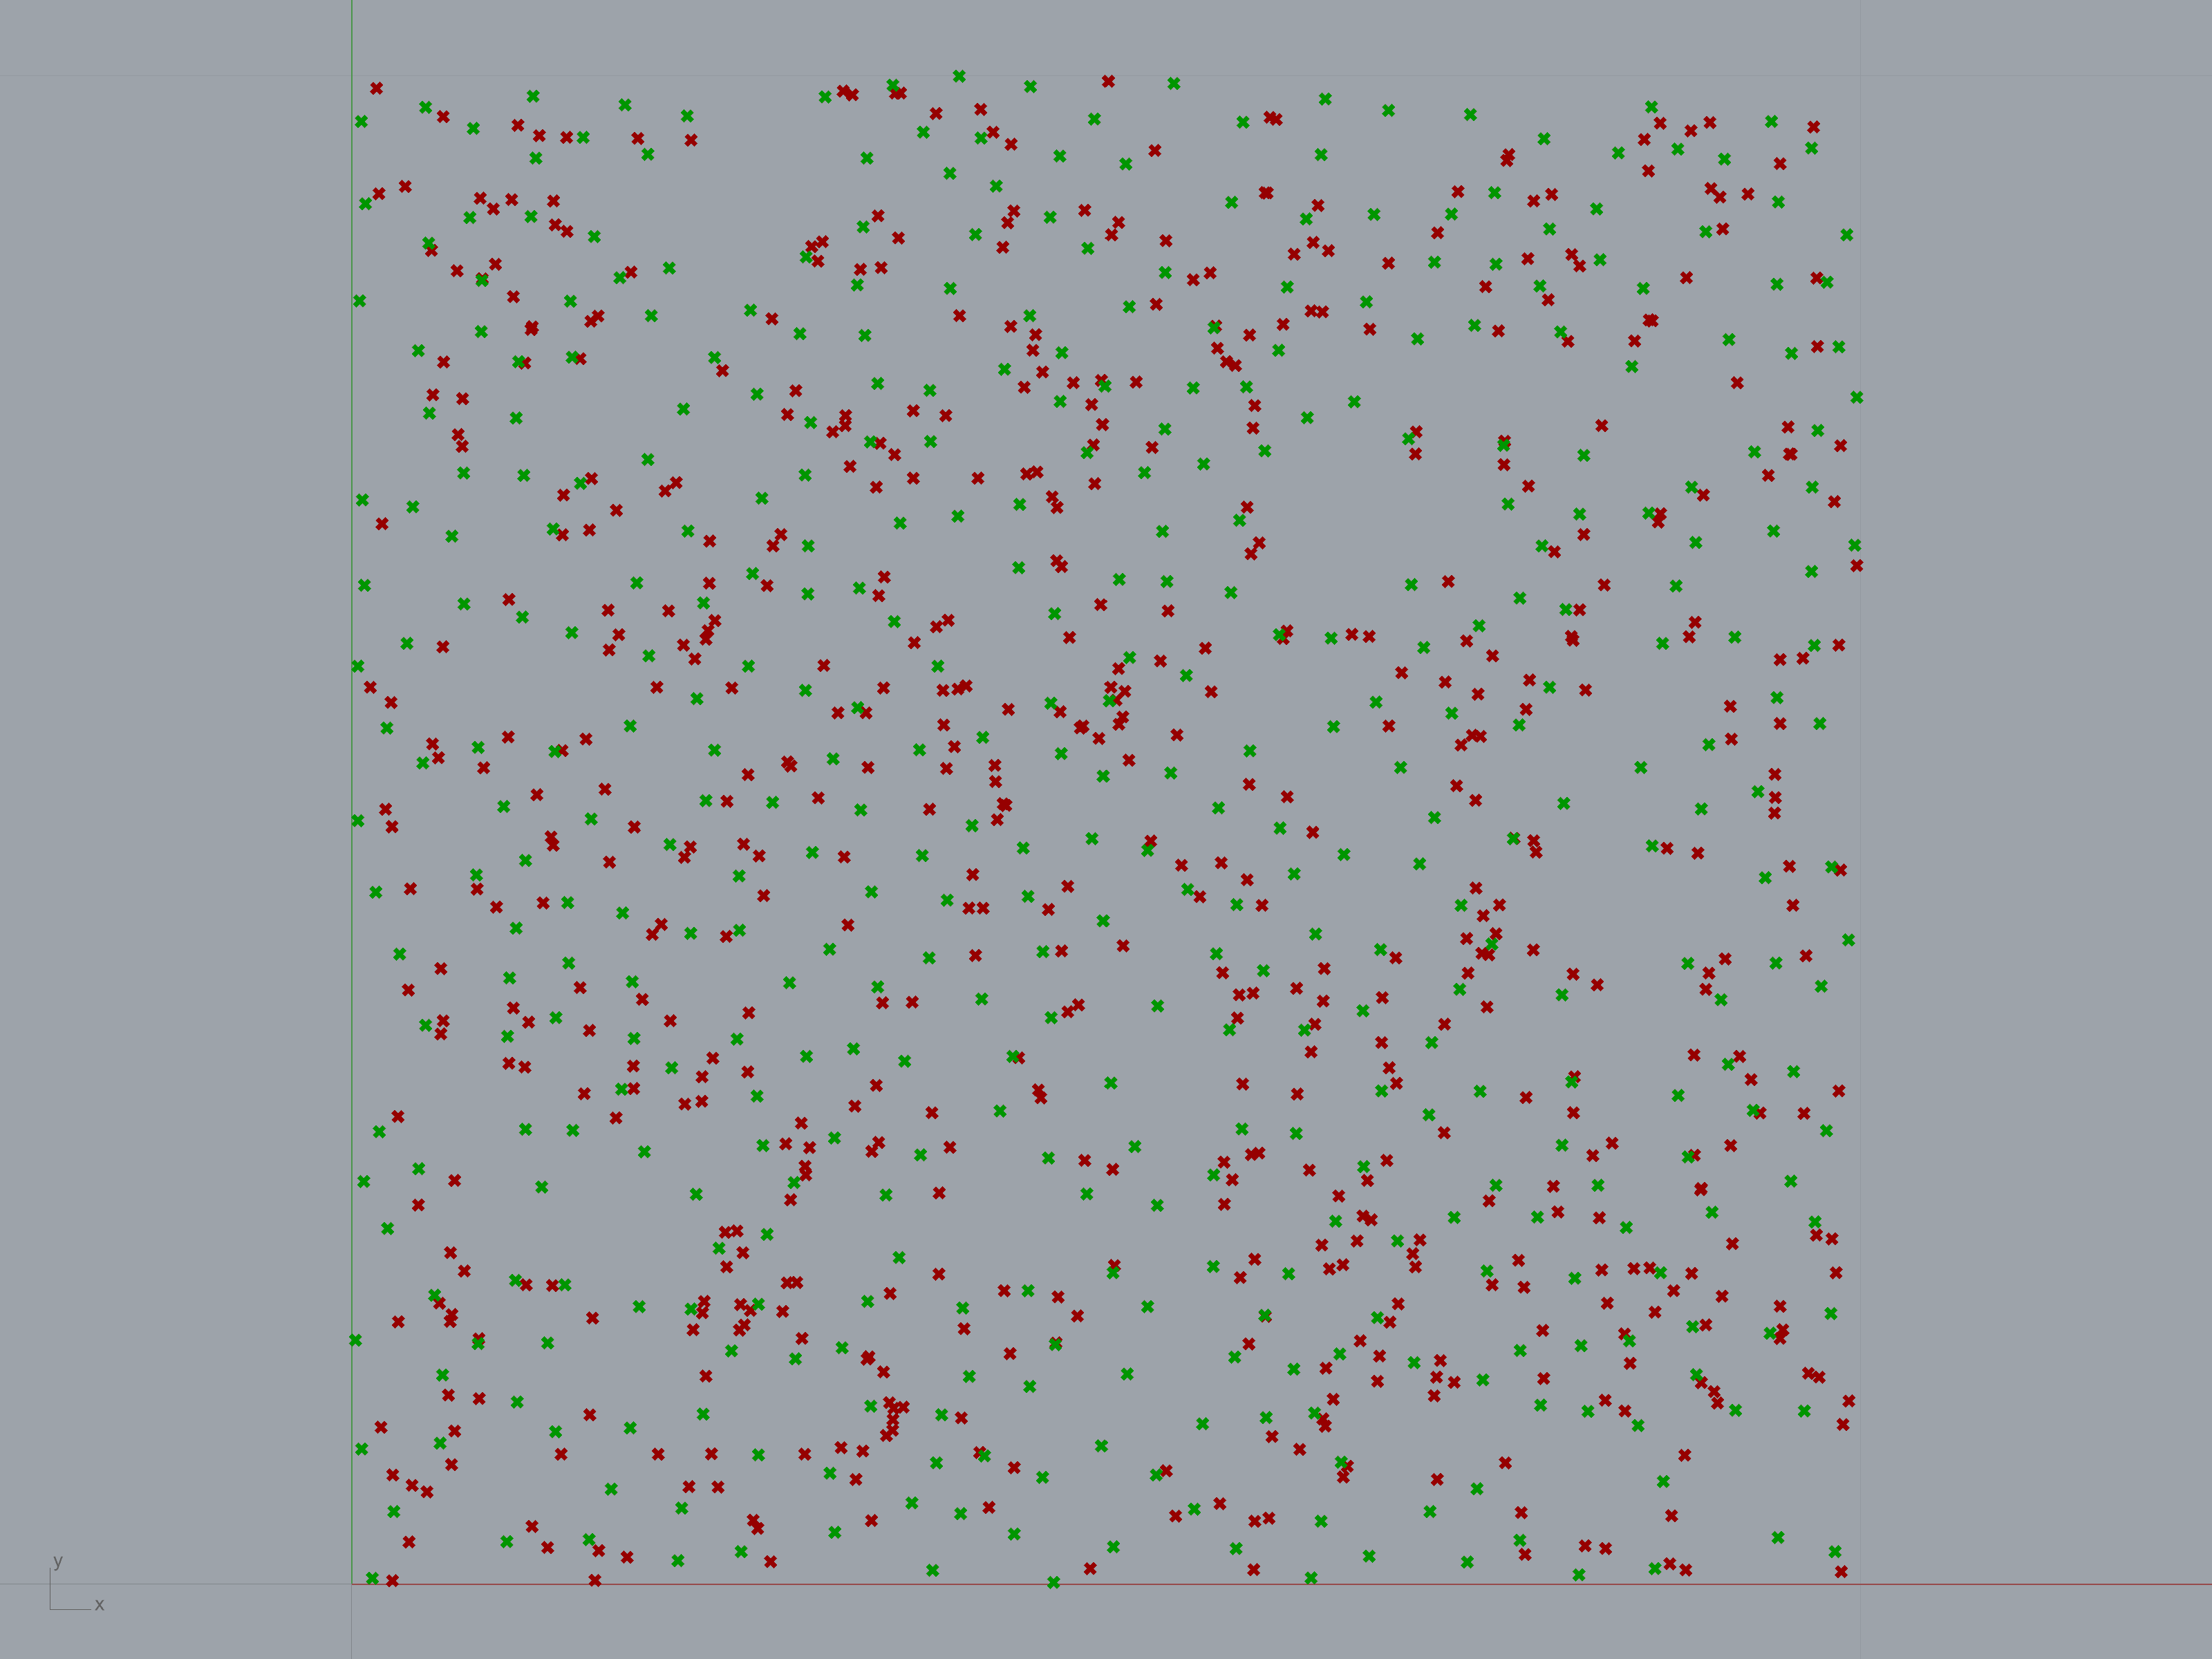
\includegraphics[height = 0.6 \linewidth]{remove-duplicate-points-capture.png}
  \caption{容差合并结果 (\keep{保留}, \remove{删除})}
  \label{fig:benchmark-result}
\end{figure}

\begin{figure}[htbp]
  \centering
  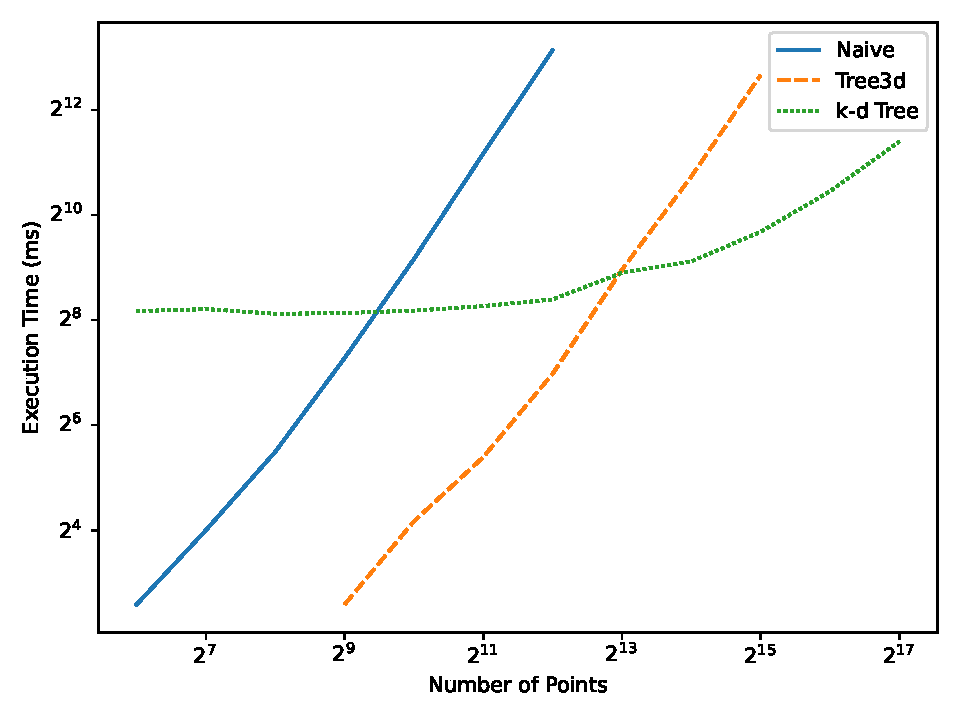
\includegraphics[height = 0.6 \linewidth]{benchmark.pdf}
  \caption{容差合并算法的性能测试结果}
  \label{fig:benchmark}
\end{figure}

\begin{table}[htbp]
  \centering
  \caption{容差合并算法的性能测试结果}
  \label{tab:benchmark}
  \begin{tabular}{ccccc}
    \toprule
    Num Points                            & Tolerance                               & \codeinline{python}{Naive} & \codeinline{csharp}{Tree3d} & \codeinline{python}{k-d Tree} \\
    \midrule
    \tablenum[table-format = 6.0]{64}     & \tablenum[table-format = 1.6]{0.125000} & \SI{6}{\milli\second}      &                             & \SI{288}{\milli\second}       \\
    \tablenum[table-format = 6.0]{128}    & \tablenum[table-format = 1.6]{0.088388} & \SI{16}{\milli\second}     &                             & \SI{296}{\milli\second}       \\
    \tablenum[table-format = 6.0]{256}    & \tablenum[table-format = 1.6]{0.062500} & \SI{45}{\milli\second}     &                             & \SI{278}{\milli\second}       \\
    \tablenum[table-format = 6.0]{512}    & \tablenum[table-format = 1.6]{0.044194} & \SI{155}{\milli\second}    & \SI{6}{\milli\second}       & \SI{281}{\milli\second}       \\
    \tablenum[table-format = 6.0]{1024}   & \tablenum[table-format = 1.6]{0.031250} & \SI{573}{\milli\second}    & \SI{18}{\milli\second}      & \SI{290}{\milli\second}       \\
    \tablenum[table-format = 6.0]{2048}   & \tablenum[table-format = 1.6]{0.022097} & \SI{2.3}{\second}          & \SI{42}{\milli\second}      & \SI{308}{\milli\second}       \\
    \tablenum[table-format = 6.0]{4096}   & \tablenum[table-format = 1.6]{0.015625} & \SI{9.0}{\second}          & \SI{126}{\milli\second}     & \SI{336}{\milli\second}       \\
    \tablenum[table-format = 6.0]{8192}   & \tablenum[table-format = 1.6]{0.011049} &                            & \SI{497}{\milli\second}     & \SI{478}{\milli\second}       \\
    \tablenum[table-format = 6.0]{16384}  & \tablenum[table-format = 1.6]{0.007813} &                            & \SI{1.7}{\second}           & \SI{555}{\milli\second}       \\
    \tablenum[table-format = 6.0]{32768}  & \tablenum[table-format = 1.6]{0.005524} &                            & \SI{6.5}{\second}           & \SI{820}{\milli\second}       \\
    \tablenum[table-format = 6.0]{65536}  & \tablenum[table-format = 1.6]{0.003906} &                            &                             & \SI{1.4}{\second}             \\
    \tablenum[table-format = 6.0]{131072} & \tablenum[table-format = 1.6]{0.002762} &                            &                             & \SI{2.7}{\second}             \\
    \bottomrule
  \end{tabular}
\end{table}

% | Num Points | Tolerance | Naive (Python) | Tree3d (C\#) | k-d Tree (Python) |
% | :--------: | :-------: | :------------: | :----------: | :---------------: |
% |     64     | 0.125000  |      6 ms      |              |      288 ms       |
% |    128     | 0.088388  |     16 ms      |              |      296 ms       |
% |    256     | 0.062500  |     45 ms      |              |      278 ms       |
% |    512     | 0.044194  |     155 ms     |     6 ms     |      281 ms       |
% |    1024    | 0.031250  |     573 ms     |    18 ms     |      290 ms       |
% |    2048    | 0.022097  |     2.3 s      |    42 ms     |      308 ms       |
% |    4096    | 0.015625  |     9.0 s      |    126 ms    |      336 ms       |
% |    8192    | 0.011049  |                |    497 ms    |      478 ms       |
% |   16384    | 0.007813  |                |    1.7 s     |      555 ms       |
% |   32768    | 0.005524  |                |    6.5 s     |      820 ms       |
% |   65536    | 0.003906  |                |              |       1.4 s       |
% |   131072   | 0.002762  |                |              |       2.7 s       |

% 已知:
% - k-d tree 由于调用了外部 python, 存在较大的通信和启动开销
% - 空白数据表示运行时间过短或过长

% 假设你是一名资深的参数化软件研究员, 你正在撰写一篇关于 Rhino 和 Grasshopper 的实际应用的中文论文. 你实现了三种点的容差合并算法, 请根据上述 benchmark 和信息, 对比分析各算法的测试结果 (不必再介绍各算法的原理), 并给这一小节取一个合适的标题. 要求语言符合学术规范.

点的容差合并算法是一种在参数化建模中常用的技术, 它可以将距离小于一定阈值的点合并为一个点, 从而简化模型的复杂度和提高运算效率.
本文实现了三种点的容差合并算法, 分别是 \codeinline{python}{Naive}, \codeinline{csharp}{Tree3d} 和 \codeinline{python}{k-d Tree}, 并在不同规模的点集上进行了测试, 测试方法如 \cref{fig:benchmark-gh} 所示, 比较了它们的运行时间和合并效果, 测试结果如 \cref{fig:benchmark-result,fig:benchmark,tab:benchmark} 所示.
下面是测试结果的分析:
\begin{itemize}
  \item \codeinline{python}{Naive} 算法是一种最简单的算法, 它遍历所有的点对, 计算它们之间的距离, 如果小于给定的容差, 则将它们合并为一个点.
        这种算法的时间复杂度是 $\Theta(n^2)$, 其中 $n$ 是点的个数.
        从表格中可以看出, 当点的个数增加时,  \codeinline{python}{Naive} 算法的运行时间呈指数增长, 当点的个数超过 \num{2048} 时, 运行时间就超过了 \SI{2}{\second}, 当点的个数达到 \num{8192} 时, 运行时间就超过了 \SI{10}{\second}.
        这说明 \codeinline{python}{Naive} 算法在处理大规模的点集时效率非常低下, 不适合用于实际应用.
  \item \codeinline{csharp}{Tree3d} 算法是一种基于空间划分的算法, 它利用了C\#语言提供的三维树结构, 将点集划分为若干个立方体区域, 然后对每个区域内的点进行容差合并.
        这种算法的时间复杂度是$\Theta(k n \log n)$, 其中 $n$ 是点的个数, $k$ 是平均每个点的近邻数量.
        从表格中可以看出, \codeinline{csharp}{Tree3d} 算法在处理不同规模的点集时都有较好的性能, 运行时间随着点的个数增加而增加, 但增长速度较慢.
        当点的个数达到 \num{32768} 时, 运行时间仍然在 \SI{6.5}{\second} 以内.
        这说明 \codeinline{csharp}{Tree3d} 算法在处理大规模的点集时效率较高, 适合用于实际应用.
  \item \codeinline{python}{k-d Tree} 算法是一种基于递归划分的算法, 它利用了 \codeinline{python}{scipy} 提供的 k-d 树结构, 将点集按照每个维度依次划分为两个子集, 然后对每个子集内的点进行容差合并.
        这种算法的时间复杂度也是$\Theta(n \log{n} + k n)$, 其中 $n$ 是点的个数, $k$ 是平均每个点的近邻数量.
        从表格中可以看出, \codeinline{python}{k-d Tree} 算法在处理不同规模的点集时都有较好的性能, 运行时间随着点的个数增加而增加, 但增长速度较慢.
        当点的个数达到 \num{131072} 时, 运行时间仍然在 \SI{2.7}{\second} 以内.
        这说明 \codeinline{python}{k-d Tree} 算法在处理大规模的点集时效率较高, 适合用于实际应用.
\end{itemize}

综上所述, 我们可以得出以下结论:
\begin{itemize}
  \item 在三种算法中, \codeinline{python}{Naive} 算法是最简单但也最低效的算法, 在处理大规模的点集时不可取.
  \item 在三种算法中, \codeinline{csharp}{Tree3d} 和 \codeinline{python}{k-d Tree} 算法都是基于空间划分或递归划分的高效算法, 在处理大规模的点集时都有较好的性能.
  \item 由于调用了外部 Python, 存在较大的通信和启动开销, 因此 \codeinline{python}{k-d Tree} 算法相比于 \codeinline{csharp}{Tree3d} 算法有一定程度上的性能损失.
\end{itemize}

% : [1](https://www.wolframalpha.com/input/?i=9+seconds+*+2%5E%28%288192-4096%29%2F2048%29)
% : [2](https://docs.microsoft.com/en-us/dotnet/api/system.windows.media.media3d.point3dcollection?view=net-5.0)
% : [3](https://docs.scipy.org/doc/scipy/reference/generated/scipy.spatial.KDTree.html)
% : [4](https://www.rhino3d.com/features/rhino-python/)
% : [5](https://developer.rhino3d.com/guides/rhinopython/python-running-scripts/)

\subsection{点集的排序}

% 为了获得稳定的合并结果, 我们需要对点集进行合理排序, 否则可能会导致合并结果的不稳定.
% 不妨定义点集上的良序算符为 $<$, 对于容差范围内的点, 保留最小的一个.
% 例如, 假设 $v_1 < v_2 < v_3$ 且 $\|v_1 - v_2\|, \|v_2 - v_3\| < t$.
% 如果按从小到大的顺序, 我们先检查 $v_1$, 那么 $v_2$ 将被删去, 而 $v_3$ 将被保留.
% 如果按从大到小的顺序我们先检查 $v_3$, 那么 $v_3$ 将被删去而 $v_2$ 将被保留; 此时再检查 $v_2$, 则 $v_2$ 被删去, $v_1$ 保留.
% 由此可见, 合并结果的稳定性取决于处理点集的顺序.
% 为了避免连环删除, 我们需要对点集进行排序, 使得点集中的点按照从小到大的顺序排列.

% 假设你是一名资深的参数化软件研究员, 你正在撰写一篇关于点的容差合并算法的论文.
% 请根据以上信息, 撰写介绍上述排序的必要性和正确性的一小节.
% 首先定义点集上的良序算符, 然后, 介绍删除重复点的方法, 再次举例说明合理排序的必要性, 最后进行总结.

点的容差合并算法的一个关键步骤是对点集进行排序, 以保证合并结果的稳定性和正确性.
在本节中, 我们将介绍我们采用的排序算法, 并证明它的必要性和有效性.

我们首先定义点集上的全序关系为 $\leqslant$, 它满足以下性质:
\begin{itemize}
  \item \emph{反对称性:} 对于任意点 $v_1, v_2$, 如果 $v_1 \leqslant v_2$ 且 $v_2 \leqslant v_1$, 则 $v_1 = v_2$.
  \item \emph{传递性:} 对于任意点 $v_1, v_2, v_3$, 如果 $v_1 \leqslant v_2$ 且 $v_2 \leqslant v_3$, 则 $v_1 \leqslant v_3$.
  \item \emph{完全性:} 对于任意点 $v_1, v_2$, 要么 $v_1 \leqslant v_2$, 要么 $v_2 \leqslant v_1$.
\end{itemize}

我们可以根据点的坐标来定义这样一个算符.
例如, 如果点的维数为 $d$, 我们可以按照字典序来比较点的坐标.
即, 对于两个点 $v_1 = (x_{11}, x_{12}, ..., x_{1d})$ 和 $v_2 = (x_{21}, x_{22}, ..., x_{2d})$, 我们有:
\begin{equation*}
  v_1 < v_2 \iff \exists i \in \{1, 2, ..., d\}, \forall j \in \{1, 2, ..., i-1\}, x_{1j} = x_{2j} \land x_{1i} < x_{2i}
\end{equation*}

这样定义的算符满足上述性质, 并且可以在 $\mathcal{O}(d)$ 的时间内比较两个点.

其次, 我们介绍如何删除重复点.
给定一个点集 $P$ 和一个容差参数 $t$, 我们的目标是找到一个子集 $Q$, 使得 $Q$ 中的任意两个点之间的距离都大于或等于 $t$, 且 $Q$ 包含了 $P$ 中所有不可删除的点.
我们称一个点是不可删除的, 如果它在容差范围内没有比它更小的点.
我们的删除方法如下:
\begin{enumerate}
  \item 对点集 $P$ 按照算符 $<$ 进行排序, 得到一个序列 $\Bqty{v_1, v_2, \dots, v_n}$.
  \item 从左到右遍历序列, 对于每个点 $v_i$, 检查它是否在容差范围内有比它更小的点.
        如果有, 则将其标记为可删除的; 如果没有, 则将其加入到子集 $Q$ 中.
  \item 返回子集 $Q$ 作为最终的合并结果.
\end{enumerate}

接下来, 我们举例说明合理排序的必要性.
假设我们有三个点 $v_1 = (0, 0)$, $v_2 = (0.5, 0)$ 和 $v_3 = (1, 0)$, 且容差参数为 $t = 0.6$.
如果我们按照从小到大的顺序处理这些点, 那么我们会得到子集 $\Bqty{v_1, v_3}$; 如果我们按照从大到小的顺序处理这些点, 那么我们会得到子集 $\Bqty{v_1}$.
可见, 处理顺序会影响合并结果的稳定性.

最后, 我们证明我们的排序方法是正确的.
即对于任意一个点集 $P$ 和一个容差参数 $t$, 我们的方法能够找到一个包含所有不可删除点的子集 $Q$.
为了证明这一点, 我们需要以下两个引理:

\begin{lem}{}{remove-duplicate-points-1}
  如果一个点是不可删除的, 那么它一定是最小的点或者它左边没有在容差范围内的点.
\end{lem}

\begin{lem}{}{remove-duplicate-points-2}
  如果一个点是可删除的, 那么它一定有一个比它更小且在容差范围内的不可删除点.
\end{lem}

\Cref{lem:remove-duplicate-points-1} 的证明很简单:
如果一个点既不是最小的点, 又有左边在容差范围内的点, 那么它就可以被这个左边的点替代, 因此是可删除的.

\Cref{lem:remove-duplicate-points-2} 的证明如下:
设一个可删除点为 $v_i$, 那么它一定有一个比它更小且在容差范围内的点 $v_j$, 其中 $j < i$. 如果 $v_j$ 是不可删除的, 那么引理成立.
如果 $v_j$ 是可删除的, 那么根据 \cref{lem:remove-duplicate-points-1}, 它一定有一个比它更小且在容差范围内的点 $v_k$, 其中 $k < j$.
我们可以重复这个过程, 直到找到一个不可删除的点为止.
这个过程一定会终止, 因为序列是有限的, 而且最小的点一定是不可删除的.

有了这两个引理, 我们就可以证明我们的方法是正确的.
设我们的方法得到的子集为 $Q$, 我们需要证明 $Q$ 包含了所有不可删除点.
对于任意一个不可删除点 $v_i$, 根据 \cref{lem:remove-duplicate-points-1}, 它一定是最小的点或者它左边没有在容差范围内的点.
如果它是最小的点, 那么它一定会被我们的方法加入到 $Q$ 中; 如果它左边没有在容差范围内的点, 那么当我们遍历到它时, 我们也会将它加入到 $Q$ 中.
因此, 对于任意一个不可删除点, 我们都能保证它在 $Q$ 中.

综上所述, 我们证明了我们的排序方法是正确的, 并且能够保证合并结果的稳定性.
